% Created 2020-09-30 Wed 15:22
% Intended LaTeX compiler: pdflatex
\documentclass[10pt,t]{beamer}
\usepackage[utf8]{inputenc}
\usepackage[T1]{fontenc}
\usepackage{graphicx}
\usepackage{grffile}
\usepackage{longtable}
\usepackage{wrapfig}
\usepackage{rotating}
\usepackage{amsmath}
\usepackage{textcomp}
\usepackage{amssymb}
\usepackage{capt-of}
\usepackage{hyperref}
\usetheme{default}
\author{C. L. Hepplewhite}
\date{\today}
\title{\large CHIRP Radiance Corrections/Offsets Connecting AIRS, SNPP, JPSS-1, and IASI}
\subtitle{\footnotesize{AIRS Virtual Science Team Meeting}}
\date{\vspace{0.1in}\footnotesize{October 2020 \vfill}}
\author{C. L. Hepplewhite\inst{1,2}, L. Larrabee Strow\inst{1,2}, and Howard Motteler\inst{2} }
\institute[UMBC]{\inst{1} UMBC Physics Dept. \and \inst{2}UMBC JCET}
\input beamer_setup
\usetheme{metropolis}
\metroset{titleformat title=allcaps}
\renewcommand{\UrlFont}{\small\tt}
\renewcommand*{\UrlFont}{\footnotesize}
\tolerance=1000
\begin{document}

\maketitle

\begin{frame}[label={sec:org80ad0c8}]{Summary}
\begin{block}{Summary}
\begin{itemize}
\item  First item
\end{itemize}

\end{block}
\end{frame}
% -----------------------------------------------------
\begin{frame}[label={sec:org6169a6e}]{One graph}

\begin{center}
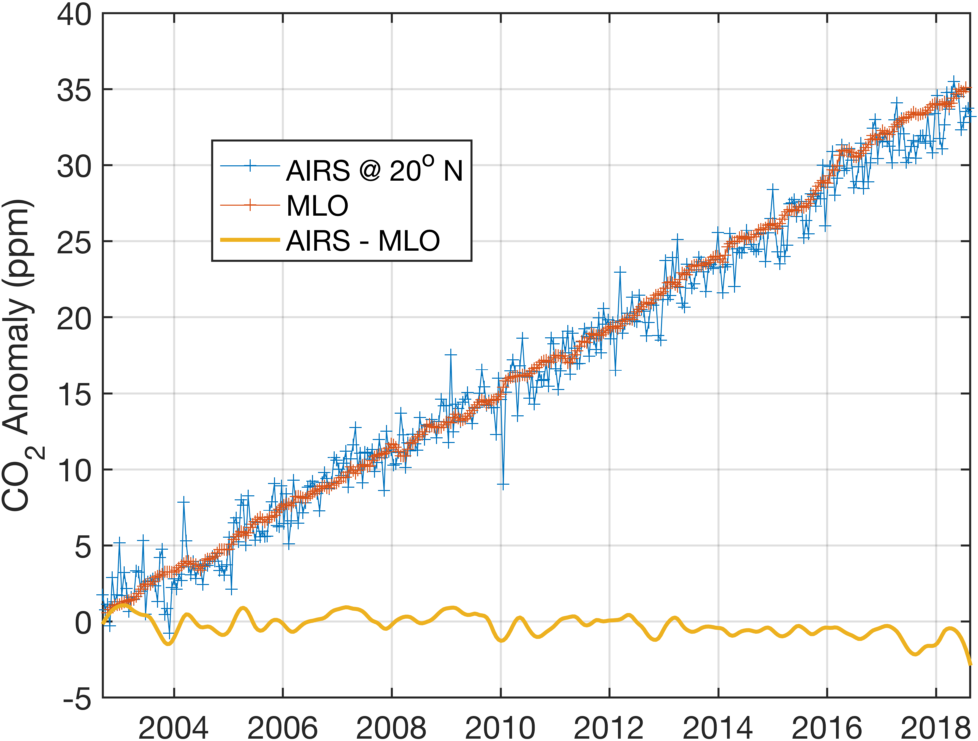
\includegraphics[width=0.8\linewidth]{./Figs/airs_vs_mlo_co2_anom_jun24.png}
\end{center}
\end{frame}
% -----------------------------------------------------

\begin{frame}[label={sec:org409cb32}]{Two}
\vspace{-0.6in}
\begin{columns}
\begin{column}{0.55\columnwidth}
\begin{block}{}
\begin{center}
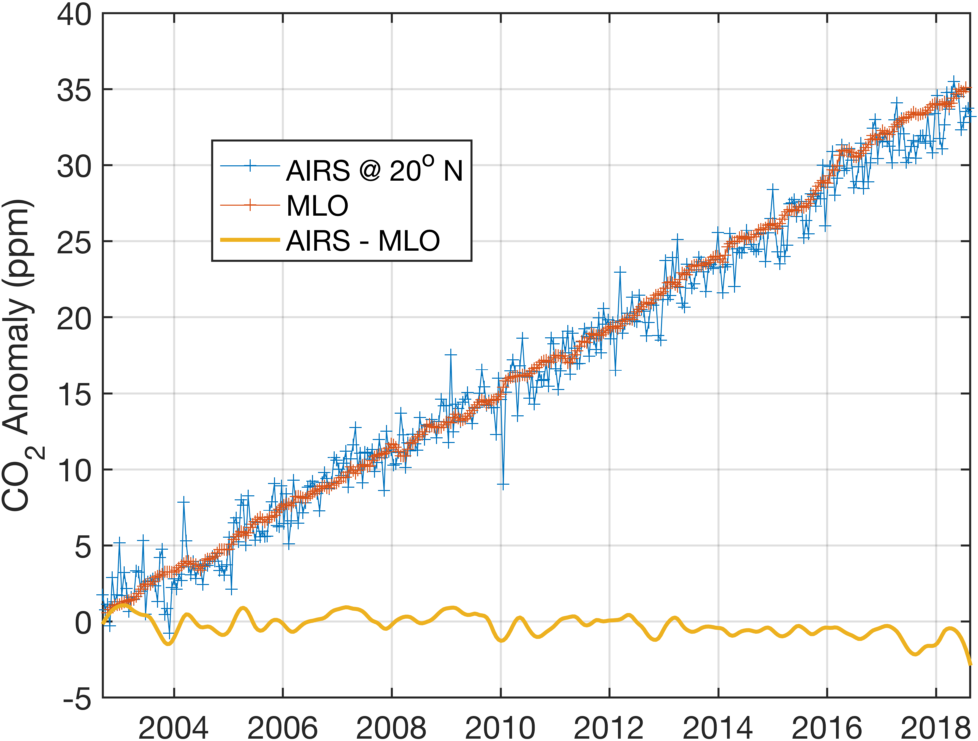
\includegraphics[width=\linewidth]{./Figs/airs_vs_mlo_co2_anom_jun24.png}
\end{center}
\end{block}
\end{column}
\end{columns}
\end{frame}
% -----------------------------------------------------

\end{document}
